
\section{Results}
\label{sec:results}

As explained in the methodology, the first step is to carry out a clustering process on the dataset in order to properly label the samples according to the classes to be used in the decision tree algorithm. Figure \ref{fig:clusters} presents a sample of the results obtained after applying the constrained \kmeans{} method, including subspacing. Recall that there are a total of 550 subspaces. Figure \ref{fig:clusters} shows three examples for each one of the subspaces considered, that is, three for each one of the 2-, 3-, and 4-feature subspace analyses. However, since it is not practical or possible to present three- or higher-dimensional plots, we display the results from a two-dimensional perspective into the the subspaces by picking 2 metrics at a time. (Note that the only cases in which this is a direct view into the clustering results are the 2-feature analysis cases.)

Some aspects of Fig.~\ref{fig:clusters} are worth discussing. Although in most plots all four clusters are clearly distinguishable, there are others in which that is not the case. In the C5-C9 and C7-C9 combinations in the 3-feature analysis, for instance, the excellent cluster has a limited presence. This is due to the influence of the lower C9 values (see Fig.~\ref{fig:data-box-plot}) on the correlations with C5 and C7. This is not necessarily a bad thing, as it helps to understand the different relationships between the various GOF metrics. In the best of cases, the combinations C1-C2 and C5-C8 in the 2- and 4-feature analysis, for instance, exhibit an almost perfect proportionality between the metrics. That means either one of the metrics in those combinations is redundant. Relationships with redundant features are those where knowledge about one of the features provides a direct view into the other. On the other hand, the combination C1-C7 in the 2-feature analysis presents an example of an irrelevant feature. We say C1 is irrelevant because it provides no insight about the outcome of C7 or that of the clusters. Identifying subspaces with redundant and irrelevant features is important because, on the one hand, the former help reduce the number of necessary features, while on the other hand, the latter can essentially be discarded because of their weak contribution to the decision making process \citep{Dy_2004_MLR}.

\begin{figure*}[ht!]
	\centering
	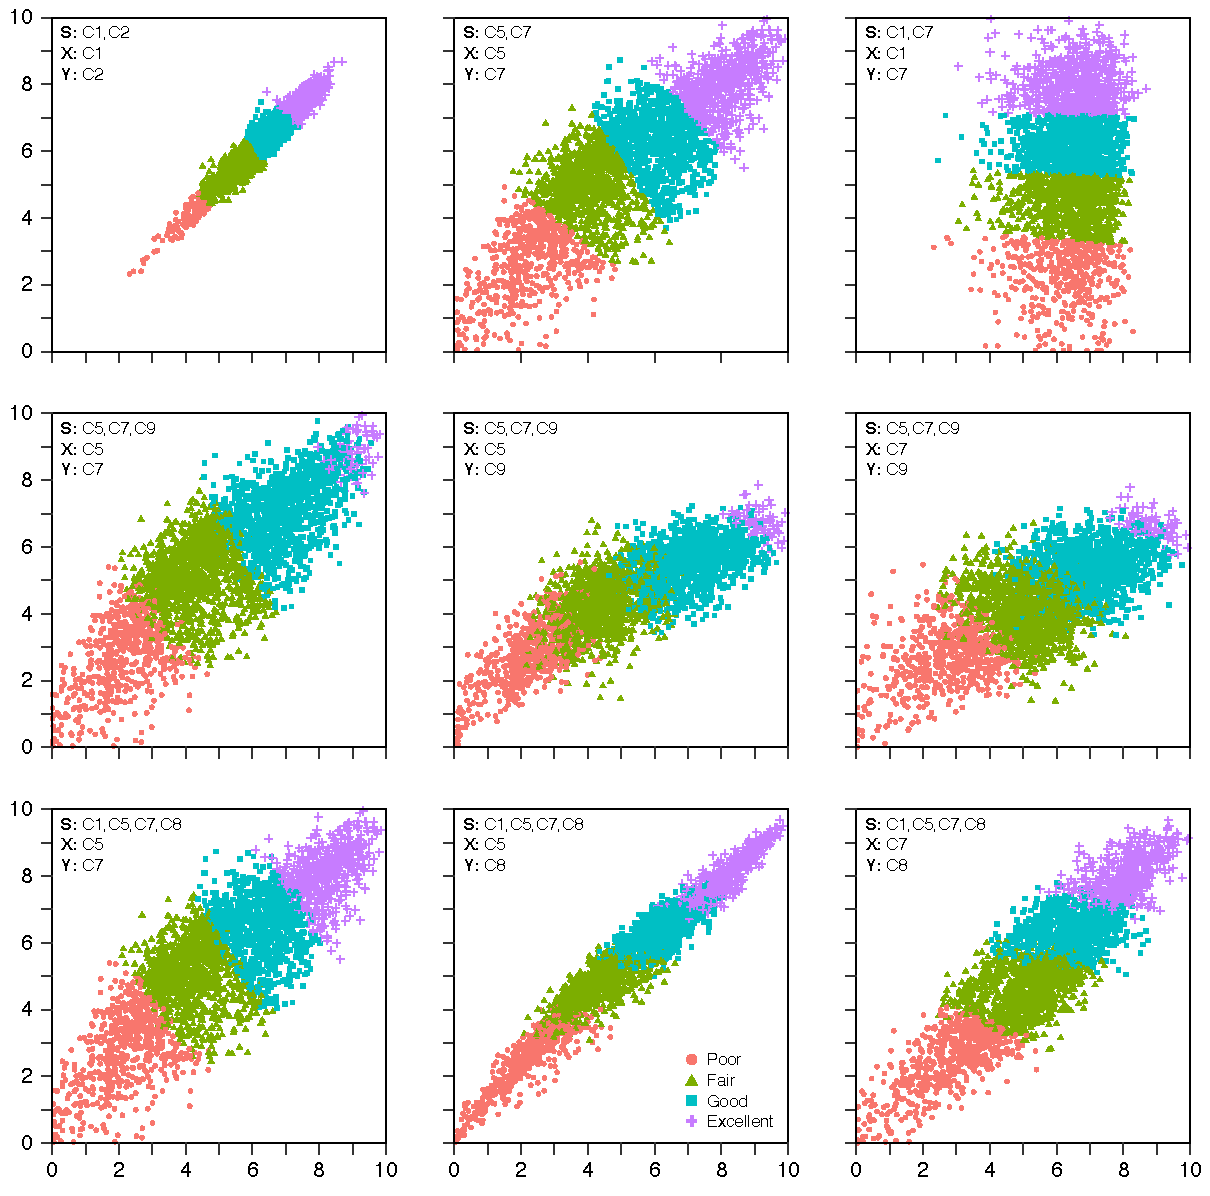
\includegraphics[width=\textwidth]{figures/pdf/figure-05}
	\caption{A sample of the results from the multi-dimensional clustering analysis showing the clusters from a two-dimensional perspective into the relationships between different GOF metrics. In each case, the labels near the upper-left corner indicate the features considered in the subspace analysis, and the features associated to the horizontal ($x$) and vertical ($y$) axes in the plot. The top, middle, and bottom rows correspond to 2-, 3-, and 4-feature subspace analyses. In each case, the poor, fair, good, and excellent clusters are indicated with circle, triangle, square, and cross symbols, respectively. The empty circles indicate the location of the artificial cannot-link stations we introduced as background knowledge to the clustering process. The color version of this figure is available only in the electronic edition.}
	\label{fig:clusters}
\end{figure*}

Figure \ref{fig:boxed-clusters} shows the statistical distribution (box-plots) of the samples once the dataset is partitioned into the four GOF validation classes. This is similar to Fig.~\ref{fig:data-box-plot}, but after the clustering process is completed. Separately, we prepared similar plots to look at the influence of the velocity models and components of motions on the results of the clustering process and, as observed before, they had no significant differences with the aggregate of all the samples in the dataset.

\begin{figure*}
	\centering
	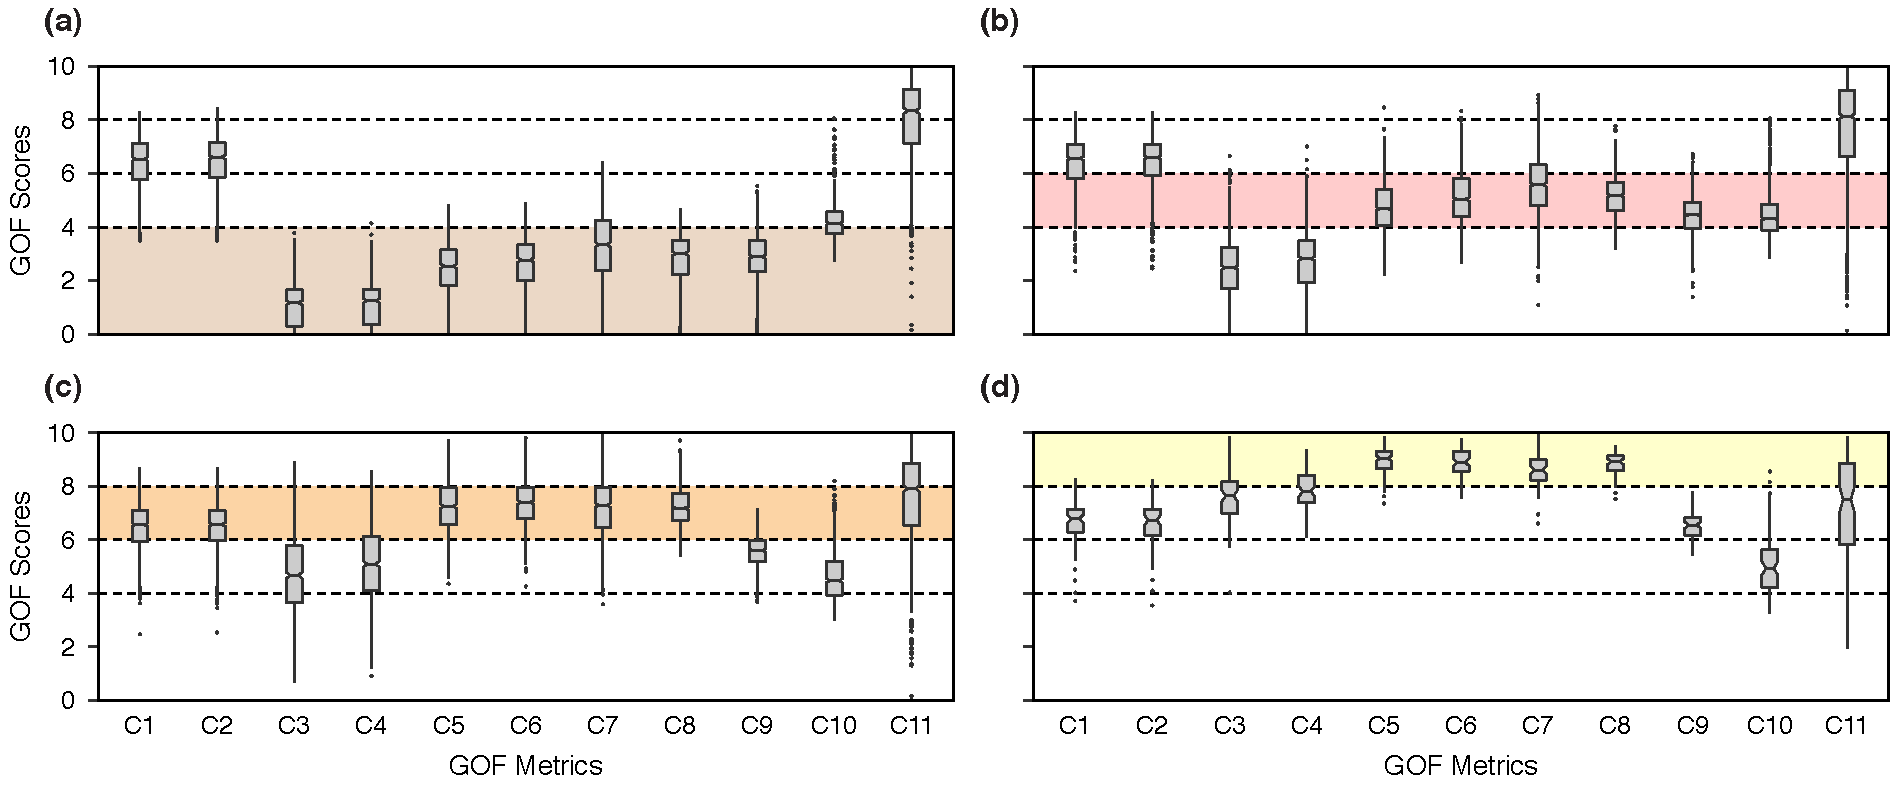
\includegraphics[width=\textwidth]{figures/pdf/figure-06}
	\caption{Statistical distribution of the dataset as partitioned into the four validation categories (poor, fair, good, excellent) after the clustering analysis. The distributions are shown in the form of box-plots for each metric (C1 through C11). In each case, the median is indicated by a notch in the box of the central quartiles, and the lines represent the interquartile range, with outliers shown as scattered dots. The color version of this figure is available only in the electronic edition.}
	\label{fig:boxed-clusters}
\end{figure*}

In total, the clustering process results in 816, 1253, 879 and 76 data samples for the poor, fair, good and excellent classes, respectively. These groups are shown in Fig.~\ref{fig:count-classes}. As it can be seen in this figure, the number of samples in the excellent class is significantly less than those in the poor, fair, and good classes. Therefore, before moving on with the decision tree analysis, it is necessary to resample the subset of the excellent class. We used the oversampling approach described in the previous section. We replicated data from the excellent class randomly by a $\times$10 factor until elevating the number of samples in this class to 760 as indicated in Fig.~\ref{fig:count-classes} with the dashed line. By common standards, an oversample rate of $\times$10 is considered acceptable \citep{Weiss_2003_JAIR}. (Arguably, we could have as well undersampled the fair class, but we deemed that unnecessary. Instead, we used a strong pruning process to prevent overfitting.) Once this process was completed we went on with the decision tree analysis. 

\begin{figure}[t]
	\centering
	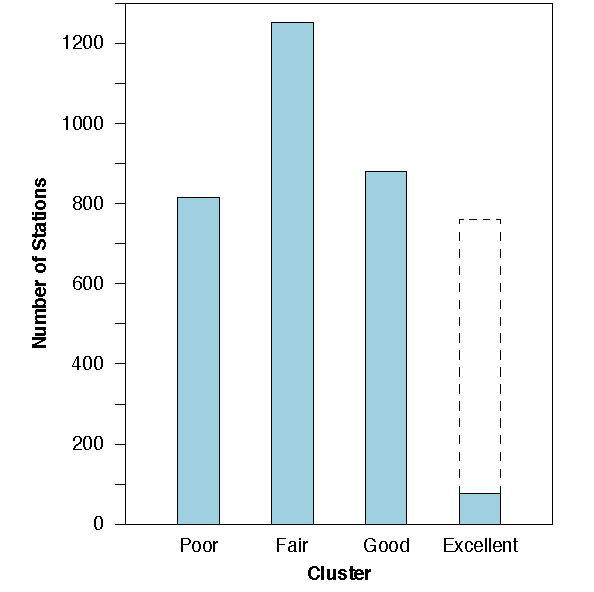
\includegraphics[width=\columnwidth]{figures/pdf/figure-07}
	\caption{Number of data samples in each class (poor, fair, good, excellent) after conducting a multi-dimensional constrained \kmeans{} clustering process using subspace analysis for 2, 3, and 4 features (GOF metrics). The dashed-line bar indicates the number of samples in the excellent class after oversampling. The color version of this figure is available only in the electronic edition.}
	\label{fig:count-classes}
\end{figure}

In total we generated 20,000 trees using the C5.0 algorithm for all possible combinations of the parameters CF and $S_{\min}$, where CF was chosen to vary between 0 and 1 at intervals of size 0.01, and $S_{\min}$ was chosen to vary between 1 and 200 at unitary intervals. Despite our choice for small intervals, the algorithm often reached recurrent tree structures for different CF and $S_{\min}$ values. Therefore, in reality, from the 20,000 combinations for which we ran the algorithm, only 66 unique trees were found. 

\begin{figure*}[t]
	\centering
	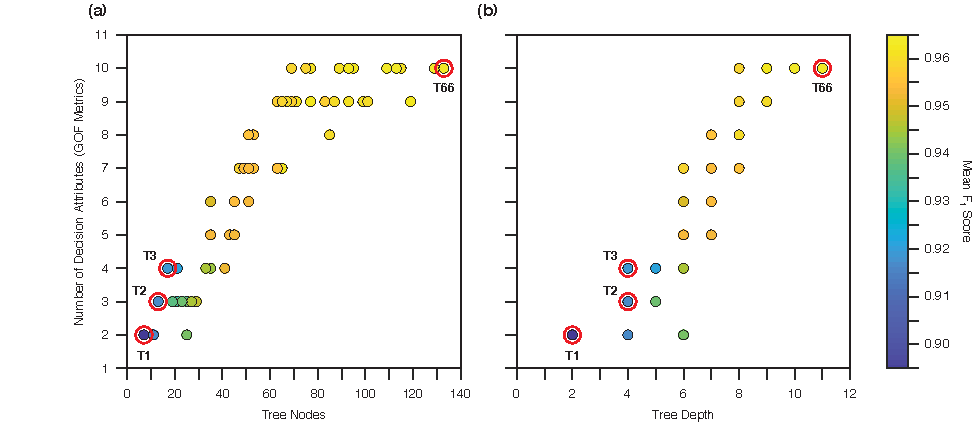
\includegraphics[width=\textwidth]{figures/pdf/figure-08}
	\caption{Accuracy of tree predictions in terms of the factor ($F_1$) from equation \ref{eq:f} as indicated by colored dots distributed with respect to the number of attributes (GOF metrics) as a function of: \textbf{(a)} the number of nodes, and \textbf{(b)} the depth of the trees. The rings around the left-most bottom dots indicate selected trees shown in Fig.~\ref{fig:trees}. The color version of this figure is available only in the electronic edition.}
	\label{fig:nodes-depth}
\end{figure*}

\begin{table}[t]
	\centering
	\caption{Confusion matrix results for decision tree T1}
	\label{tab:t1:confusion}
	\small
	\begin{tabular}{cccccc}
		& 		& \multicolumn{4}{c}{Prediction}\\ 
		\cline{3-6}
		&   	& P  	& F     & G  	& E 	\\
		\cline{2-6}
		\parbox[t]{2mm}{\multirow{4}{*}{\rotatebox[origin=c]{90}{Actual}}}  
		& P 	& 242 	& 11 	& 0     & 0    	\\
		& F 	& 13 	& 313   & 16    & 0    	\\
		& G 	& 0 	& 42    & 207   & 15   	\\
		& E 	& 0 	& 0     & 23    & 231	\\ 
		\cline{2-6}
	\end{tabular}
\end{table}

\begin{table}[t]
	\centering
	\caption{Confusion matrix results for decision tree T3}
	\label{tab:t3:confusion}
	\small
	\begin{tabular}{cccccc}
		& 		& \multicolumn{4}{c}{Prediction}\\ 
		\cline{3-6}
		&   	& P  	& F     & G  	& E 	\\
		\cline{2-6}
		\parbox[t]{2mm}{\multirow{4}{*}{\rotatebox[origin=c]{90}{Actual}}}  
		& P 	& 248 	& 14 	& 0     & 0    	\\
		& F 	& 7 	& 343   & 18    & 0    	\\
		& G 	& 0 	& 9 	& 221   & 33   	\\
		& E 	& 0 	& 0     & 7    	& 213	\\ 
		\cline{2-6}
	\end{tabular}
\end{table}

For each one of these unique trees, we computed the effectiveness factor $F_1$ from equation (\ref{eq:f}), and extracted the total number of nodes in the trees and their depth. Figure \ref{fig:nodes-depth} shows the results of $F_1$ for all the trees and its distribution in terms of the number of attributes used in the trees as a function of the number of nodes and the depth of each tree. Recall that we are interested in finding a sequence of decisions (represented by disjunctive decision nodes in a tree) that can lead to good GOF predictions (i.e, high values of $F_1$) using a reduced number of attributes (GOF metrics). In general, all the trees obtained with the C5.0 algorithm are good in terms of the effectiveness factor ($F_1$ values close to 1). Then our choice comes down to using a reduced number of metrics. Having several trees with 2, 3, and 4 metrics (as opposed to 11), the following factor in the decision is choosing trees with algorithms using a small number of steps to reach the prediction. This is given by a combination between the depth of the tree and the number of nodes in the tree (i.e., trees with low complexity).

Based on these criteria, we selected three candidate trees: T1, T2, and T3. These trees are shown in Fig.~\ref{fig:trees}. T1 is the simplest of the three, and T2 and T3 share some of their topology on the right-hand side. T3 is the most complex of them. More complex trees tend to be deeper, have more nodes, and employ more attributes. This leads to higher $F_1$ values, but they may not necessarily be more practical. In total T1, T2, and T3 use 2, 3 and 4 attributes respectively. All coincide in the use of the total energy (C4) and response spectra (C8) as key metrics. T2 adds peak acceleration (C5), and T3 adds peak velocity (C5) to the previous metrics.

\begin{figure*}
	\centering
	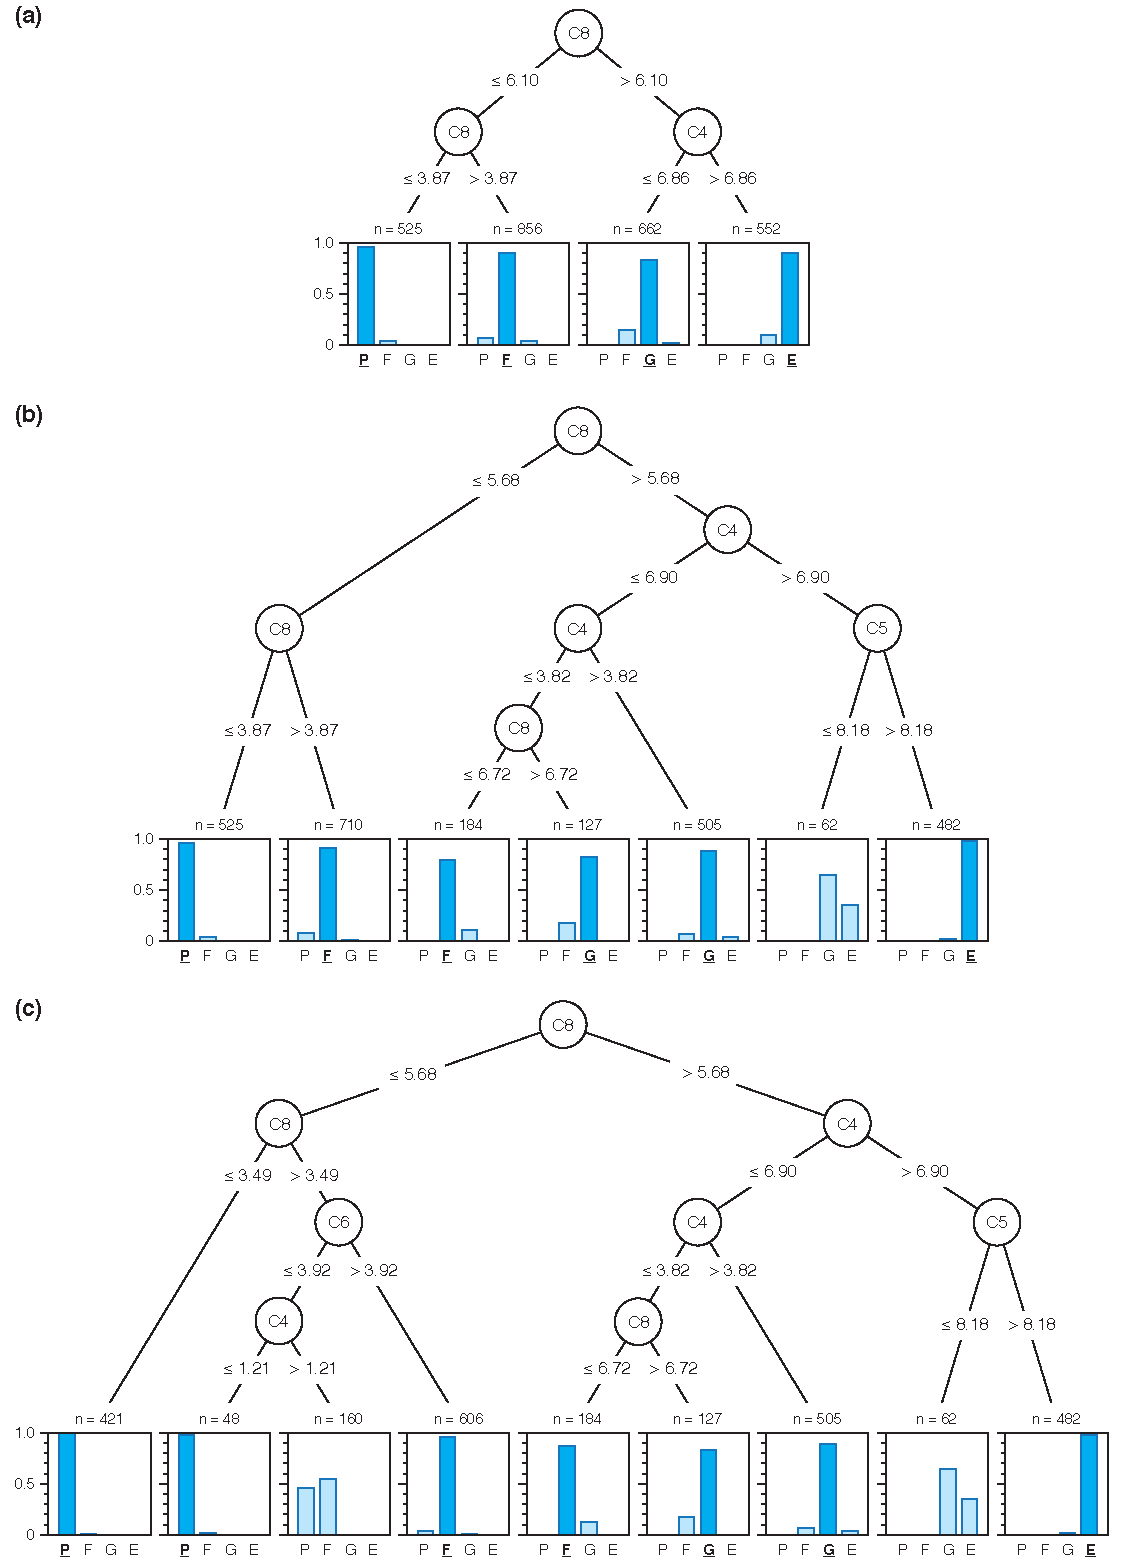
\includegraphics[width=0.86\textwidth]{figures/pdf/figure-09}
	\caption{Selected trees \textbf{(a)} T1, \textbf{(b)} T2, and \textbf{(c)} T3. In each case the decision nodes of the trees contain the code corresponding to the metric (see Table \ref{tab:metrics}) used and the branches beneath each node show the limit value to be used to select the next level in the tree. At the bottom, normalized histograms are shown to indicate the distribution of the samples at each leaf-node according to the validation classes with codes P, F, G, and E for poor, fair, good, and excellent, respectively. At the top of each histogram is the total count of samples at the corresponding leaf node. The histograms highlight the dominant validation class. The color version of this figure is available only in the electronic edition.}
	\label{fig:trees}
\end{figure*}

\begin{table}[t]
	\centering
	\caption{T1 precision, recall, and $F_1$ values per class}
	\label{tab:t1:f1}
	\small
	\begin{tabular}{lccc}
	Class   & $P$	& $R$  	& $F_1$ \\ 
	\hline
	P 		& 0.96 	& 0.95 	& 0.95 	\\
	F 		& 0.92 	& 0.86 	& 0.88 	\\
	G 		& 0.78 	& 0.84 	& 0.81 	\\
	E 		& 0.91 	& 0.94 	& 0.92 	\\
	\hline
	Mean 	&		&		& 0.90	\\
	\end{tabular}
\end{table}

\begin{table}[t]
	\centering
	\caption{T3 precision, recall, and $F_1$ values per class}
	\label{tab:t3:f1}
	\small
	\begin{tabular}{lccc}
	Class   & $P$	& $R$  	& $F_1$ \\ 
	\hline
	P 		& 0.95 	& 0.97 	& 0.95 	\\
	F 		& 0.93 	& 0.93 	& 0.93 	\\
	G 		& 0.84 	& 0.89 	& 0.86 	\\
	E 		& 0.96 	& 0.86 	& 0.91 	\\
	\hline
	Mean 	&		&		& 0.91	\\
	\end{tabular}
\end{table}

At the bottom of each tree in Fig.~\ref{fig:trees} are the histograms of the data that land on each leaf node. (Note that the count of samples here is done based on the training dataset.) The decision tree assigns the final validation category based on the dominant class in each leaf. As such, the samples in the second leaf-node from the right in T3 are categorized as good despite a significant portion of them being excellent. This is a natural trade-off embedded in the use of decision trees which actually results in more effective trees. 

The actual effectiveness (i.e., the average $F_1$ values shown in Fig.~\ref{fig:nodes-depth}), however, is measured based on the testing dataset. Recall that $F_1$ depends on the number of true predictions and false predictions measured by the confusion matrix and the precision and recall factors. Tables \ref{tab:t1:confusion} and \ref{tab:t3:confusion} show the confusion matrices for T1 and T3, respectively; and Tables \ref{tab:t1:f1} and \ref{tab:t3:f1} show the corresponding results for $P$, $R$, and $F_1$. As it can be seen in the Tables \ref{tab:t1:confusion} and \ref{tab:t3:confusion}, both trees lead to strong diagonal confusion matrices, meaning that the classification into poor, fair, good and excellent is well defined. The differences between both matrices are actually minor and small with respect to their diagonal values, and the $F_1$ values in Tables \ref{tab:t1:f1} and \ref{tab:t3:f1} are all near to or above 0.9. The values obtained for tree T2 are consistent with this.

The final selection of a preferred tree, then, comes down to reducing the complexity. We favor tree T1 because it is based only in three decision steps, and two GOF metrics, C4: energy, and C8: response spectra.

